%% Standard LaTeX article wrapper for compiling the shared English manuscript body
%% without requiring any publisher-specific document class.
\documentclass[11pt,a4paper]{article}
\usepackage[top=26mm,bottom=26mm,left=26mm,right=26mm]{geometry}
\usepackage{amsmath,amssymb,amsfonts,amsthm,mathtools}
\usepackage{tikz}
\usepackage[title]{appendix}
\usepackage{booktabs}
\usepackage[hidelinks]{hyperref}
\hypersetup{colorlinks=true,linkcolor=black,citecolor=black,urlcolor=blue}

\newtheorem{theorem}{Theorem}[section]
\newtheorem{lemma}[theorem]{Lemma}
\newtheorem{proposition}[theorem]{Proposition}
\newtheorem{corollary}[theorem]{Corollary}
\theoremstyle{definition}
\newtheorem{remark}[theorem]{Remark}
\newtheorem{question}[theorem]{Question}
\newtheorem{problem}[theorem]{Problem}

\newcommand{\Dom}{\mathcal{D}}
\newcommand{\Crit}{\operatorname{Crit}}
\DeclareUrlCommand\lean{\urlstyle{tt}\def\UrlBreaks{\do\_}}
\newcommand{\MaxLC}{26}
\newcommand{\MinNonLC}{27}
\newcommand{\MaxOrder}{27}
\newcommand{\TotalTreesLC}{447\,672\,596}
\newcommand{\TotalTreesAll}{1\,198\,738\,056}
\newcommand{\MaxJumpValue}{1.04}

\newcommand{\AuthorEmail}{skdl3965@gmail.com}


\title{Unimodality of domination polynomials of forests with upper domination gap at most four}
\author{Chanu Hong\\{\normalsize Gyeongin National University of Education, Incheon, Republic of Korea}\\{\normalsize \texttt{\AuthorEmail}}}
\date{November 2026}

\begin{document}
\maketitle

\begin{abstract}
Let $\gamma(G)$ and $\Gamma(G)$ denote the domination number and the upper
domination number of a graph $G$. Beaton and Schoonhoven (2024) proved that the
domination polynomial of a tree $T$ is unimodal whenever
$\Gamma(T)-\gamma(T)\le2$. We prove that the domination polynomial of every
forest $F$ with $\Gamma(F)-\gamma(F)\le4$ is unimodal. More generally, a
forest of order $n$ without isolated vertices whose domination polynomial is
not unimodal satisfies $n\le6\lceil(h+1)^2/4\rceil-h-16$, where
$h=\Gamma(F)-\gamma(F)$; in particular, the domination polynomial of such a
forest is unimodal whenever $h\le\sqrt{2n/3}-1$. The proofs rest on a short argument showing that
a dominating set $S$ of a bipartite graph $G$ has at most $2\alpha(G)-|S|$
critical vertices, and on a variance estimate which shows that the average
number of critical vertices of the dominating sets of size $j$ cannot
increase by more than two when $j$ increases by one, provided that
$j-\gamma(F)\ge\lceil(h+1)^2/4\rceil$. The case
$\Gamma-\gamma=4$ relies in addition on an exhaustive computation, which shows
that the domination polynomial of every tree with at most $\MaxLC$ vertices is
log-concave, whereas exactly one tree with $\MinNonLC$ vertices is not. The main analytic steps have been formalised in Lean~4.

\medskip\noindent\textbf{Keywords:} Domination polynomial, Unimodality, Log-concavity, Upper domination number, Forest, Bipartite graph.

\noindent\textbf{2020 Mathematics Subject Classification:} 05C69, 05C31, 05C05.
\end{abstract}

%% Shared body of the manuscript (used by both journal wrappers), part 1.
\section{Introduction}\label{sec:intro}

All graphs in this paper are finite and simple. A set $S$ of vertices of a
graph $G$ is \emph{dominating} if every vertex outside $S$ has a neighbour
in $S$. Writing $d_j(G)$ for the number of dominating sets of $G$ of
cardinality $j$, the \emph{domination polynomial} of a graph $G$ of order $n$ is
\[
  D(G,x)=\sum_{j=0}^{n} d_j(G)\,x^j .
\]
A sequence $(d_0,\dots,d_n)$ of nonnegative numbers is \emph{unimodal} if
$d_0\le d_1\le\dots\le d_m\ge d_{m+1}\ge\dots\ge d_n$ for some index $m$, and
\emph{log-concave} if $d_j^2\ge d_{j-1}d_{j+1}$ for $1\le j\le n-1$; a
polynomial is called unimodal or log-concave if its coefficient sequence is.
Alikhani and Peng~\cite{AP} conjectured that the domination polynomial of
every graph is unimodal. The conjecture is open, even for trees.

Much of what is known is recorded in
\cite{BB22,BO,BS,DHP,GZ,Omar}. Beaton and Brown~\cite{BB22} proved unimodality for
graphs of sufficiently large minimum degree and exhibited a graph on nine
vertices whose domination polynomial is not log-concave. Burcroff and
O'Brien~\cite{BO} showed that the coefficients of $D(G,x)$ are nonincreasing
from about $(n+\Gamma(G))/2$ onwards, where $\Gamma(G)$, the \emph{upper
domination number}, is the largest cardinality of a minimal dominating set.
For trees, Beaton and Schoonhoven~\cite{BS} constructed an infinite family
with non-log-concave domination polynomials, and proved that $D(T,x)$ is
unimodal for every tree $T$ with $\Gamma(T)-\gamma(T)<3$, where $\gamma$
denotes the domination number. We call $\Gamma(G)-\gamma(G)$ the
\emph{upper domination gap} of~$G$; graphs with gap zero are the
well-dominated graphs.

The purpose of this paper is to extend the result of Beaton and Schoonhoven
in three directions: from trees to forests, from gap at most two to gap at
most four, and from a fixed gap to a gap that may grow with the order.

\begin{theorem}\label{thm:gapfour-intro}
Let $F$ be a forest with $\Gamma(F)-\gamma(F)\le 4$. Then the domination
polynomial of $F$ is unimodal.
\end{theorem}

For larger gaps we obtain unimodality for all but finitely many forests of
each given gap, apart from isolated vertices, which only multiply the
domination polynomial by a power of~$x$.

\begin{theorem}\label{thm:criterion-intro}
Let $F$ be a forest of order $n$ with $h=\Gamma(F)-\gamma(F)$, and put
$K_h=\lceil (h+1)^2/4\rceil$.
\begin{enumerate}
\item[\textup{(i)}] If $n-\gamma(F)\ge 3K_h-7$, then $D(F,x)$ is unimodal.
\item[\textup{(ii)}] If $F$ has no isolated vertices and $D(F,x)$ is not
unimodal, then $h\ge 3$ and $n\le 6K_h-h-16$.
\item[\textup{(iii)}] In particular, if $F$ has no isolated vertices and
$3h^2+4h-19\le 2n$, then $D(F,x)$ is unimodal.
\end{enumerate}
\end{theorem}

Part~(iii) applies, for instance, whenever
$\Gamma(F)-\gamma(F)\le\sqrt{2n/3}-1$. The bound in part~(ii) equals $5$ for
$h=3$, $22$ for $h=4$ and $33$ for $h=5$. The case $h=3$ of
Theorem~\ref{thm:gapfour-intro} follows from it by inspecting a single
forest, the star $K_{1,4}$. The case $h=4$ needs the domination polynomials of
forests with at most $22$ vertices, and here we rely on a computation which
establishes more than is needed and may be of independent interest.

\begin{theorem}\label{thm:smalltrees-intro}
\begin{enumerate}
\item[\textup{(i)}] The domination polynomial of every tree with at most $\MaxLC$
vertices is log-concave. Consequently, the domination polynomial of every
forest all of whose components have at most $\MaxLC$ vertices is log-concave,
and hence unimodal.
\item[\textup{(ii)}] Among the $751\,065\,460$ trees with $\MinNonLC$ vertices
there is exactly one whose domination polynomial is not log-concave.
\end{enumerate}
\end{theorem}

The exceptional tree is shown in Figure~\ref{fig:U}; its domination polynomial
is unimodal. Thus $\MinNonLC$ is the smallest order of a tree with a
non-log-concave domination polynomial. The trees of Beaton and
Schoonhoven~\cite{BS} have $9k+4$ vertices and were shown there to be
non-log-concave for $k\ge4$, that is, from order $40$ on. Further trees and
graphs with non-log-concave domination polynomials were recently found
in~\cite{DHP} with the machine-learning software PatternBoost; the trees
displayed there have $32$ and $58$ vertices. The same paper constructs trees
whose domination polynomials fail to be log-concave at arbitrarily many
indices. That the smallest order is $\MinNonLC$ parallels the situation for
the independence polynomial, for which Kadrawi and Levit~\cite{KL} found that
log-concavity first fails for trees of order~$26$.

\subsection*{Method}
For a dominating set $S$, a vertex $v\in S$ is \emph{critical} if
$S\setminus\{v\}$ is not dominating; let $a(S)$ be the number of critical
vertices of $S$. Counting pairs of nested dominating sets of consecutive
sizes shows that $d_{j-1}\le d_j$ holds exactly when the average of $a(S)$
over the dominating sets of size $j$ is at least $2j-n-1$; this observation
is the basis of~\cite{BS}. Beaton and Schoonhoven proved that every
dominating set $S$ of a tree $T$ satisfies
\begin{equation}\label{eq:BS-bounds}
  2\gamma(T)-|S|\;\le\; a(S)\;\le\; 2\Gamma(T)-|S| ,
\end{equation}
and deduced that the coefficients increase up to about $(n+2\gamma)/3$ and
decrease from about $(n+2\Gamma)/3$ on, which leaves at most one undetermined
step when $\Gamma-\gamma\le2$.

Our contribution has two parts. First, we give a short proof of the upper
bound in~\eqref{eq:BS-bounds} that works for every bipartite graph and
establishes the bound $|S|+a(S)\le 2\alpha(G)$, where $\alpha$ is the
independence number (Lemma~\ref{lem:upper}). The original proof for trees
in~\cite{BS} is long and relies on a reconfiguration argument. As a
by-product, the decreasing segment and the upper bound on the average order
of dominating sets from~\cite{BS} extend to all bipartite graphs
(Corollary~\ref{cor:segments}). Second, and more importantly, we control the
window that the two monotone segments leave open. Writing $c_j$ for the
average of $a(S)$ over dominating sets of size $j$, a \emph{valley}
$d_{i-1}\ge d_i<d_{i+1}$ forces $c_{i+1}-c_i>2$ (Lemma~\ref{lem:valley}),
whereas a covariance inequality between consecutive ranks, combined with
\eqref{eq:BS-bounds} and an elementary variance bound, gives
$c_{j}-c_{j-1}\le 2$ as soon as $j-\gamma\ge\lceil (h+1)^2/4\rceil$
(Lemma~\ref{lem:jump}). When the order is large compared with the gap, this
range covers the whole window. Some restriction on $j$ is necessary here: we
show that $c_{j+1}-c_j<2(j-\gamma)+1$ for every forest and that this bound is
sharp for trees, so that the differences $c_{j+1}-c_j$ can exceed two and are
in fact unbounded (Proposition~\ref{prop:jumps}).

\subsection*{Verification}
Theorem~\ref{thm:gapfour-intro} for gap four and
Theorem~\ref{thm:smalltrees-intro} depend on exhaustive computations, which
were carried out by two programs that use different tree generators and separate implementations of equivalent
forms of the same domination-polynomial recurrence; see
Appendix~\ref{app:computation}. In addition, the main analytic statements
have been formalised in Lean~4 with Mathlib~\cite{Lean,Mathlib}; the precise
scope of the formalisation is described in Appendix~\ref{app:lean}. The
programs, their outputs and the Lean sources accompany this paper as
supplementary material.

\subsection*{Organisation}
Section~\ref{sec:prelim} collects basic facts. Section~\ref{sec:critical}
contains the two bounds on $a(S)$ and their direct consequences.
Section~\ref{sec:jump} studies the averages $c_j$, and
Section~\ref{sec:unimodal} proves Theorem~\ref{thm:criterion-intro} and the
cases of Theorem~\ref{thm:gapfour-intro} with gap at most three.
Section~\ref{sec:small} deals with small trees and completes the proof of
Theorem~\ref{thm:gapfour-intro}. Section~\ref{sec:remarks} contains remarks
and questions.

\section{Preliminaries}\label{sec:prelim}

Let $G$ be a graph with vertex set $V$ and order $n=|V|$. For $v\in V$ we
write $N[v]$ for the closed neighbourhood of $v$, so that $S\subseteq V$ is
dominating if and only if $N[u]\cap S\ne\emptyset$ for every $u\in V$. A
dominating set is \emph{minimal} if none of its proper subsets is dominating.
We write $\gamma(G)$ for the minimum cardinality of a dominating set,
$\Gamma(G)$ for the maximum cardinality of a minimal dominating set, and
$\alpha(G)$ for the maximum cardinality of an independent set. Let
$\Dom_j(G)$ be the family of dominating sets of cardinality $j$, so that
$d_j=d_j(G)=|\Dom_j(G)|$; we put $d_j=0$ for $j<0$ and for $j>n$.

For a dominating set $S$ let
\[
  \Crit(S)=\{v\in S:\ S\setminus\{v\}\text{ is not dominating}\},\qquad
  a(S)=|\Crit(S)| .
\]
A vertex $v\in S$ is critical if and only if it has a \emph{private witness}:
a vertex $u$ with $N[u]\cap S=\{v\}$. A dominating set $S$ is minimal if and
only if $a(S)=|S|$.

\begin{lemma}\label{lem:basic}
Let $G$ be a graph of order $n$.
\begin{enumerate}
\item[\textup{(i)}] $d_j>0$ if and only if $\gamma(G)\le j\le n$.
\item[\textup{(ii)}] If $S\subseteq U$ are dominating sets, then
$\Crit(U)\subseteq\Crit(S)$.
\item[\textup{(iii)}] For $1\le j\le n$,
\begin{equation}\label{eq:incidence}
  (n-j+1)\,d_{j-1}=\sum_{S\in\Dom_j(G)}\bigl(j-a(S)\bigr).
\end{equation}
\end{enumerate}
\end{lemma}

\begin{proof}
(i) Every superset of a dominating set is dominating.

(ii) Let $v\in\Crit(U)$. If $v\notin S$, then $S\subseteq U\setminus\{v\}$,
so $U\setminus\{v\}$ would be dominating. Hence $v\in S$, and
$S\setminus\{v\}\subseteq U\setminus\{v\}$ is not dominating.

(iii) Count the pairs $(S',S)$ with $S'\in\Dom_{j-1}(G)$, $S\in\Dom_j(G)$ and
$S'\subset S$. Each $S'$ extends to exactly $n-j+1$ sets $S$, and each $S$
contains exactly $j-a(S)$ dominating subsets of size $j-1$.
\end{proof}

The next two facts are standard; we include the short proofs.

\begin{lemma}[Ore~\cite{Ore}]\label{lem:ore}
Let $G$ be a graph of order $n$ without isolated vertices. The complement of
every minimal dominating set of $G$ is dominating. In particular
$n\ge\gamma(G)+\Gamma(G)$.
\end{lemma}

\begin{proof}
Let $M$ be a minimal dominating set and $v\in M$, with private witness $u$.
If $u\ne v$, then $u\notin M$ (otherwise $N[u]\cap M\supseteq\{u,v\}$), so
$v$ has a neighbour outside $M$. If $u=v$, then $v$ has no neighbour in $M$,
and, not being isolated, has a neighbour outside $M$. Hence $V\setminus M$
dominates every vertex of $M$. Taking $|M|=\Gamma(G)$ gives
$\gamma(G)\le n-\Gamma(G)$.
\end{proof}

\begin{lemma}\label{lem:isolates}
Let $G$ be a graph with exactly $r$ isolated vertices and let $G^{\circ}$ be
obtained from $G$ by deleting them. Then
\[
  D(G,x)=x^{r}D(G^{\circ},x),\qquad \gamma(G)=\gamma(G^{\circ})+r,\qquad
  \Gamma(G)=\Gamma(G^{\circ})+r .
\]
In particular $G$ and $G^{\circ}$ have the same upper domination gap and the
same value of $|V|-\gamma$, and $D(G,x)$ is unimodal if and only if
$D(G^{\circ},x)$ is.
\end{lemma}

\begin{proof}
Every dominating set of $G$ contains all isolated vertices, and removing them
is a bijection between the dominating sets of $G$ and those of $G^{\circ}$
which lowers the size by $r$ and preserves minimality.
\end{proof}

\section{Critical vertices in forests and in bipartite graphs}\label{sec:critical}

The first bound is due to Beaton and Schoonhoven~\cite[Lemma~5]{BS} for
trees. We give a self-contained proof, which follows their idea of removing
a deepest non-critical vertex and applies verbatim to forests.

\begin{lemma}\label{lem:lower}
Let $S$ be a dominating set of a forest $F$. Then
$|S|+a(S)\ge 2\gamma(F)$.
\end{lemma}

\begin{proof}
We use induction on $|S|$. If every vertex of $S$ is critical, then
$|S|+a(S)=2|S|\ge2\gamma(F)$; this covers the case $|S|=\gamma(F)$. Assume
that $S\setminus\Crit(S)\ne\emptyset$. Root each component of $F$ at one of
its vertices, define the depth of a vertex as its distance from the root of
its component, and choose $v\in S\setminus\Crit(S)$ of maximum depth. The
set $S'=S\setminus\{v\}$ is dominating. We claim that
\begin{equation}\label{eq:one-more}
  a(S')\le a(S)+1 .
\end{equation}
Then $|S'|+a(S')\le|S|+a(S)$, and the induction hypothesis applied to $S'$
finishes the proof.

By Lemma~\ref{lem:basic}(ii), $\Crit(S)\subseteq\Crit(S')$. Suppose
that~\eqref{eq:one-more} fails, and let $x_1\ne x_2$ be vertices of
$\Crit(S')\setminus\Crit(S)$. For $i=1,2$ choose a private witness $u_i$ of
$x_i$ with respect to $S'$, so that $N[u_i]\cap S'=\{x_i\}$. Since $x_i$ is
not critical in $S$, we have $N[u_i]\cap S=\{x_i,v\}$. In particular
$u_1\ne u_2$, both $u_i$ lie in $N[v]$, and $x_i\in N[u_i]$. Moreover
$x_i\in S\setminus\Crit(S)$, so the depth of $x_i$ is at most the depth of
$v$ by the choice of~$v$.

Fix $i$. If $u_i=v$, then $x_i$ is a neighbour of $v$ whose depth does not
exceed that of $v$; hence $v$ is not a root and $x_i$ is the parent of $v$.
If $u_i\ne v$, then $u_i$ is a neighbour of $v$. It cannot be a child of
$v$, because every vertex of $N[u_i]\setminus\{v\}$ would then be deeper than
$v$, whereas $x_i\in N[u_i]\setminus\{v\}$. Hence $u_i$ is the parent of $v$.

As $u_1\ne u_2$, we may assume that $u_1=v$ and that $u_2=p$ is the parent of
$v$. By the first case $x_1=p$, so $p\in S'$. But then
$p\in N[u_2]\cap S'=\{x_2\}$, that is, $x_2=p=x_1$, a contradiction.
\end{proof}

The lower bound of Lemma~\ref{lem:lower} does not extend to bipartite
graphs: in the cycle $C_4$ a set $S$ of three vertices has $a(S)=0$, while
$2\gamma(C_4)-|S|=1$. The upper bound, in contrast, holds for every bipartite
graph.

\begin{lemma}\label{lem:upper}
Let $S$ be a dominating set of a bipartite graph $G$. Then
\[
  |S|+a(S)\le 2\alpha(G).
\]
\end{lemma}

\begin{proof}
For each $v\in\Crit(S)$ fix a private witness $w(v)$, so that
$N[w(v)]\cap S=\{v\}$. The map $w$ is injective, since $w(v)$ determines $v$.
Let
\[
  E=\{v\in\Crit(S): w(v)=v\},\qquad B=\Crit(S)\setminus E,\qquad W=w(B).
\]
If $v\in B$, then $w(v)\notin S$, because a vertex of $S$ belongs to its own
closed neighbourhood. Hence $W\cap S=\emptyset$ and $|W|=|B|$.

No vertex of $E$ has a neighbour in $S\cup W$. Indeed, let $v\in E$. As
$N[v]\cap S=\{v\}$, the vertex $v$ has no neighbour in $S$. If $v$ were
adjacent to $w(u)$ for some $u\in B$, then $v\in N[w(u)]\cap S=\{u\}$, which
is impossible because $u\notin E$.

Let $V(G)=X\sqcup Y$ be a bipartition of $G$ and put
\[
  I_X=\bigl((S\cup W)\cap X\bigr)\cup(E\cap Y),\qquad
  I_Y=\bigl((S\cup W)\cap Y\bigr)\cup(E\cap X).
\]
Both sets are independent: there are no edges inside $X$ or inside $Y$, and
no edges between $E$ and $S\cup W$. Since $E\subseteq S$ and $W\cap
S=\emptyset$,
\[
  2\alpha(G)\ge|I_X|+|I_Y|=|S\cup W|+|E|=|S|+|B|+|E|=|S|+a(S). \qedhere
\]
\end{proof}

A maximum independent set is a minimal dominating set, so
$\alpha(G)\le\Gamma(G)$ for every graph $G$. Conversely, applying
Lemma~\ref{lem:upper} to a minimal dominating set $M$ of a bipartite graph,
for which $a(M)=|M|$, gives $|M|\le\alpha(G)$. This reproves the classical
fact~\cite{CFPT} that
\begin{equation}\label{eq:alpha-Gamma}
  \Gamma(G)=\alpha(G)\qquad\text{for every bipartite graph } G,
\end{equation}
and shows that Lemma~\ref{lem:upper} contains the upper bound
in~\eqref{eq:BS-bounds}, which is \cite[Lemma~15]{BS}.

\begin{corollary}\label{cor:twosided}
Every dominating set $S$ of a forest $F$ satisfies
\begin{equation}\label{eq:twosided}
  2\gamma(F)-|S|\;\le\;a(S)\;\le\;2\Gamma(F)-|S| .
\end{equation}
\end{corollary}

The monotone segments of~\cite[Theorems~6 and~16]{BS} and the bounds on the
average order of dominating sets of~\cite[Theorem~18]{BS} follow at once,
now for forests and, on the upper side, for bipartite graphs. Let
$\operatorname{avd}(G)$ denote the average cardinality of a dominating set
of~$G$.

\begin{corollary}\label{cor:segments}
Let $G$ be a graph of order $n$ and let $1\le j\le n$.
\begin{enumerate}
\item[\textup{(i)}] If $G$ is a forest and $3j\le n+2\gamma(G)+1$, then
$d_{j-1}\le d_j$. Moreover $\operatorname{avd}(G)\ge(n+2\gamma(G))/3$.
\item[\textup{(ii)}] If $G$ is bipartite and $3j\ge n+2\alpha(G)+1$, then
$d_{j-1}\ge d_j$. Moreover $\operatorname{avd}(G)\le(n+2\alpha(G))/3$.
\end{enumerate}
\end{corollary}

\begin{proof}
By~\eqref{eq:incidence} and Lemma~\ref{lem:lower},
$(n-j+1)d_{j-1}\le(2j-2\gamma(G))d_j$, which is at most $(n-j+1)d_j$ when
$3j\le n+2\gamma(G)+1$. Similarly, Lemma~\ref{lem:upper} gives
$(n-j+1)d_{j-1}\ge(2j-2\alpha(G))d_j\ge(n-j+1)d_j$ when
$3j\ge n+2\alpha(G)+1$. Summing~\eqref{eq:incidence} over $j$ gives the
identity $\sum_S(|S|-a(S))=\sum_S(n-|S|)$ of Beaton and Brown~\cite{BB21},
where $S$ runs over all dominating sets; that is,
$2\operatorname{avd}(G)=n+\overline{a}$, where $\overline a$ is the average of
$a(S)$ over all dominating sets. Inserting $a(S)\ge2\gamma(G)-|S|$,
respectively $a(S)\le2\alpha(G)-|S|$, and solving for
$\operatorname{avd}(G)$ gives the two bounds.
\end{proof}

For bipartite graphs, part~(ii) improves on the threshold of order
$(n+\Gamma(G))/2$ that holds for all graphs~\cite{BO}, since
$(n+2\Gamma(G))/3\le(n+\Gamma(G))/2$.


%% Shared body of the manuscript, part 2.
\section{The average number of critical vertices}\label{sec:jump}

Throughout this section $G$ is a graph of order $n\ge1$ and
$\gamma=\gamma(G)$. For $\gamma\le j\le n$ the family $\Dom_j(G)$ is
nonempty, and we write $c_j$ and $v_j$ for the mean and the variance of
$a(S)$ when $S$ is chosen uniformly at random from $\Dom_j(G)$:
\[
  c_j=\frac1{d_j}\sum_{S\in\Dom_j(G)}a(S),\qquad
  v_j=\frac1{d_j}\sum_{S\in\Dom_j(G)}\bigl(a(S)-c_j\bigr)^2 .
\]
In this notation the identity~\eqref{eq:incidence} reads
\begin{equation}\label{eq:mean}
  j-c_j=(n-j+1)\,\frac{d_{j-1}}{d_j}\qquad(\gamma\le j\le n).
\end{equation}
In particular $j-c_j>0$ for $\gamma<j\le n$, and $d_{j-1}\le d_j$ if and only
if $c_j\ge 2j-n-1$.

\begin{lemma}\label{lem:valley}
Let $\gamma<i<n$. If $d_{i-1}\ge d_i<d_{i+1}$, then $c_{i+1}-c_i>2$.
\end{lemma}

\begin{proof}
By~\eqref{eq:mean}, $c_i=i-(n-i+1)d_{i-1}/d_i\le 2i-n-1$ and, as $n-i>0$,
$c_{i+1}=i+1-(n-i)d_i/d_{i+1}>2i+1-n$.
\end{proof}

\begin{lemma}\label{lem:cov}
For $\gamma<j\le n$,
\[
  (j-c_j)\,(c_j-c_{j-1})\le v_j .
\]
\end{lemma}

\begin{proof}
Consider again the pairs $(S',S)$ with $S'\in\Dom_{j-1}(G)$,
$S\in\Dom_j(G)$ and $S'\subset S$. By Lemma~\ref{lem:basic}(ii),
$a(S)\le a(S')$ for each such pair. Summing over all pairs, and using that
each $S$ occurs in $j-a(S)$ pairs and each $S'$ in $n-j+1$ pairs, we get
\[
  \sum_{S\in\Dom_j(G)}\bigl(j-a(S)\bigr)\,a(S)\;\le\;
  (n-j+1)\sum_{S'\in\Dom_{j-1}(G)}a(S') .
\]
The left-hand side equals $d_j\bigl((j-c_j)c_j-v_j\bigr)$, and the right-hand
side equals $(n-j+1)d_{j-1}c_{j-1}=d_j(j-c_j)c_{j-1}$ by~\eqref{eq:mean}.
Dividing by $d_j$ gives the claim.
\end{proof}

For an integer $h\ge0$ we say that $G$ satisfies condition $(\mathrm{H}_h)$ if
\begin{equation}\label{eq:H}
  2\gamma-|S|\;\le\;a(S)\;\le\;2\gamma+2h-|S|
  \qquad\text{for every dominating set $S$ of $G$.}
\end{equation}
By Corollary~\ref{cor:twosided}, every forest $F$ satisfies $(\mathrm{H}_h)$
with $h=\Gamma(F)-\gamma(F)$. We put
\[
  K_h=\left\lceil\frac{(h+1)^2}{4}\right\rceil .
\]

\begin{lemma}\label{lem:jump}
Let $G$ satisfy $(\mathrm{H}_h)$. Then $c_j-c_{j-1}\le 2$ for every $j$ with
$\gamma+K_h\le j\le n$.
\end{lemma}

\begin{proof}
Fix such a $j$; note that $j>\gamma$ because $K_h\ge1$. Put $L=2\gamma-j$ and
$x=c_j-L$. By~\eqref{eq:H}, $L\le a(S)\le L+2h$ for every $S\in\Dom_j(G)$, so
$0\le x\le 2h$. Averaging the pointwise inequality
$(a(S)-L)(L+2h-a(S))\ge0$ over $\Dom_j(G)$ gives
\begin{equation}\label{eq:variance}
  v_j\le x\,(2h-x) .
\end{equation}
Since $j-c_j=2(j-\gamma)-x$, we have the identity
\[
  2(j-c_j)-x(2h-x)=\bigl(x-(h+1)\bigr)^2+4(j-\gamma)-(h+1)^2 ,
\]
whose right-hand side is nonnegative because $j-\gamma\ge K_h\ge(h+1)^2/4$.
Together with Lemma~\ref{lem:cov} and~\eqref{eq:variance} this yields
$(j-c_j)(c_j-c_{j-1})\le v_j\le 2(j-c_j)$, and $j-c_j>0$.
\end{proof}

\section{Unimodality}\label{sec:unimodal}

\begin{theorem}\label{thm:main}
Let $G$ be a graph of order $n\ge1$ that satisfies $(\mathrm{H}_h)$ for some
integer $h\ge0$. If
\begin{equation}\label{eq:condition}
  n-\gamma(G)\ge 3K_h-7 ,
\end{equation}
then $D(G,x)$ is unimodal.
\end{theorem}

\begin{proof}
Let $\gamma=\gamma(G)$ and $A=\lfloor(n+2\gamma+1)/3\rfloor
=\gamma+\lfloor(n-\gamma+1)/3\rfloor$. As in the proof of
Corollary~\ref{cor:segments}(i), which uses only the lower bound
in~\eqref{eq:H}, we have $d_{j-1}\le d_j$ whenever $1\le j\le n$ and $j\le A$.
Condition~\eqref{eq:condition} is equivalent to
$\lfloor(n-\gamma+1)/3\rfloor\ge K_h-2$, that is, to
\begin{equation}\label{eq:A}
  A+2\ge\gamma+K_h .
\end{equation}

Suppose that $(d_0,\dots,d_n)$ is not unimodal. Then there are indices $k<i$
with $d_k>d_{k+1}$ and $d_i<d_{i+1}$; choose $k$ minimal and then $i$ minimal.
By the minimality of $i$ we have $d_{i-1}\ge d_i$, both when $i=k+1$ and when
$i>k+1$. The strict descent at $k$ shows that $k+1>A$, hence $i\ge k+1\ge
A+1\ge\gamma+1$, and $i<n$ because $d_{i+1}>0$. Lemma~\ref{lem:valley}
gives $c_{i+1}-c_i>2$. On the other hand $i+1\ge A+2\ge\gamma+K_h$
by~\eqref{eq:A}, so Lemma~\ref{lem:jump} gives $c_{i+1}-c_i\le2$, a
contradiction.
\end{proof}

\begin{proof}[Proof of Theorem~\ref{thm:criterion-intro}]
(i) This is Theorem~\ref{thm:main} together with
Corollary~\ref{cor:twosided}.

(ii) Let $F$ be a forest without isolated vertices such that $D(F,x)$ is not
unimodal, and write $\gamma=\gamma(F)$ and $K=K_h$. By~(i),
$n-\gamma\le 3K-8$. By Lemma~\ref{lem:ore}, $n\ge\gamma+\Gamma(F)=2\gamma+h$,
that is, $\gamma\le(n-\gamma)-h$. Therefore
\[
  n=(n-\gamma)+\gamma\le 2(n-\gamma)-h\le 6K-h-16 .
\]
Since $K_0=K_1=1$ and $K_2=3$, the right-hand side is at most $0$ when
$h\le2$, which is impossible. Hence $h\ge3$.

(iii) Since $K_h\le\bigl((h+1)^2+3\bigr)/4$, we have
$6K_h-h-16\le(3h^2+4h-20)/2$. If $2n\ge3h^2+4h-19$, then $n>6K_h-h-16$, and
$D(F,x)$ is unimodal by~(ii).
\end{proof}

\begin{corollary}\label{cor:gapthree}
Let $F$ be a forest with $\Gamma(F)-\gamma(F)\le3$. Then $D(F,x)$ is
unimodal.
\end{corollary}

\begin{proof}
By Lemma~\ref{lem:isolates} we may assume that $F$ has no isolated vertices.
Suppose that $D(F,x)$ is not unimodal. By
Theorem~\ref{thm:criterion-intro}(ii) the gap is $h=3$, so $K_h=4$,
$n\le5$, and $n\ge2\gamma(F)+3$ by Lemma~\ref{lem:ore}. Hence $\gamma(F)=1$
and $n=5$: some vertex is adjacent to the other four, and, $F$ being a
forest, $F$ is the star $K_{1,4}$. A dominating set of $K_{1,4}$ either
contains the centre or consists of the four leaves, so
\[
  D(K_{1,4},x)=x(1+x)^4+x^4=x+4x^2+6x^3+5x^4+x^5 ,
\]
which is unimodal. This contradiction proves the corollary.
\end{proof}

For gap at most two, Corollary~\ref{cor:gapthree} extends the theorem of
Beaton and Schoonhoven~\cite[Corollary~17]{BS} from trees to forests; the case
of gap three is new already for trees.

\section{Small trees and the case of gap four}\label{sec:small}

\subsection{Log-concavity for trees with at most \texorpdfstring{$\MaxLC$}{26} vertices}

\begin{theorem}\label{thm:small}
The domination polynomial of every tree with at most $\MaxLC$ vertices is
log-concave.
\end{theorem}

\begin{proof}
This is the result of an exhaustive computation over the $\TotalTreesLC$
isomorphism classes of trees with at most $\MaxLC$ vertices. The algorithms,
the completeness checks and the two independent implementations are described
in Appendix~\ref{app:computation}.
\end{proof}

To pass from trees to forests we use the classical fact that log-concavity is
preserved by products; see, for example, Stanley's survey~\cite{Stanley}. A
sequence $(a_k)_{k\in\mathbb Z}$ of nonnegative numbers with finitely many
nonzero terms has \emph{no internal zeros} if its support is an interval.

\begin{lemma}\label{lem:product}
Let $P$ and $Q$ be polynomials whose coefficient sequences are nonnegative,
log-concave and without internal zeros. Then the coefficient sequence of
$PQ$ has the same three properties.
\end{lemma}

\begin{proof}
Let $(a_k)$, $(b_k)$ and $(c_k)$ be the coefficient sequences of $P$, $Q$ and
$PQ$, extended by zero to all integer indices. A nonnegative log-concave
sequence $(a_k)$ without internal zeros satisfies
\begin{equation}\label{eq:tp2}
  a_i\,a_j\ge a_{i-1}\,a_{j+1}\qquad\text{for all } i\le j ,
\end{equation}
because, when the right-hand side is positive, the ratios $a_k/a_{k-1}$ are
positive and nonincreasing for $i\le k\le j+1$. Expanding the products shows
that
\[
  c_k^2-c_{k-1}c_{k+1}=\sum_{i<j}
  \bigl(a_i a_{j-1}-a_{i-1}a_j\bigr)\bigl(b_{k-j+1}b_{k-i}-b_{k-j}b_{k-i+1}\bigr),
\]
which is the Cauchy--Binet formula for a $2\times2$ minor of a product of two
matrices. Both factors of each summand are nonnegative by~\eqref{eq:tp2}.
Finally, the support of $(c_k)$ is the sumset of two intervals, hence an
interval.
\end{proof}

\begin{corollary}\label{cor:smallforest}
Let $F$ be a forest all of whose components have at most $\MaxLC$ vertices.
Then $D(F,x)$ is log-concave, and in particular unimodal.
\end{corollary}

\begin{proof}
The domination polynomial of a disjoint union is the product of the
domination polynomials of the components, and $D(K_1,x)=x$. By
Lemma~\ref{lem:basic}(i) the coefficient sequence of every domination
polynomial is nonnegative without internal zeros. The claim follows from
Theorem~\ref{thm:small} and Lemma~\ref{lem:product}, since a nonnegative
log-concave sequence without internal zeros is unimodal.
\end{proof}

\begin{proof}[Proof of Theorem~\ref{thm:gapfour-intro}]
For gap at most three this is Corollary~\ref{cor:gapthree}. Let $F$ be a
forest with $\Gamma(F)-\gamma(F)=4$; by Lemma~\ref{lem:isolates} we may
assume that $F$ has no isolated vertices. If $D(F,x)$ were not unimodal,
then $F$ would have at most $6K_4-4-16=22$ vertices by
Theorem~\ref{thm:criterion-intro}(ii), contradicting
Corollary~\ref{cor:smallforest}.
\end{proof}

\begin{remark}\label{rem:boundary}
The proof for gap four uses Theorem~\ref{thm:small} only for trees with at
most $22$ vertices, of which there are $9\,114\,285$. The forests actually
concerned are fewer: there are exactly $1\,290\,927$ isomorphism classes of
forests without isolated vertices that have gap four and satisfy
$n-\gamma\le13$ (and therefore have at most $22$ vertices); these are the
forests of gap four not covered by Theorem~\ref{thm:criterion-intro}(i). The
number is obtained from the joint distribution of the order, $\gamma$ and
$\Gamma$ over trees, since all three parameters are additive over components
(supplementary material).
\end{remark}

\subsection{The smallest tree that is not log-concave}

Let $k_1,\dots,k_r$ be nonnegative integers, and let $T(k_1,\dots,k_r)$ be
the tree obtained from a vertex $v_0$ with neighbours $v_1,\dots,v_r$ by attaching to each
$v_i$ exactly $k_i$ pendant paths on three vertices, each joined to $v_i$ by
one of its end vertices. This tree has $1+r+3\sum_i k_i$ vertices, and the
trees $T_k$ of Beaton and Schoonhoven~\cite{BS} are the trees $T(k,k,k)$.
Let $U$ be the tree with $27$ vertices obtained from $T(2,2,3)$ by adding a
path on two new vertices and joining one of them to $v_0$; see
Figure~\ref{fig:U}.

\begin{figure}[ht]
\centering
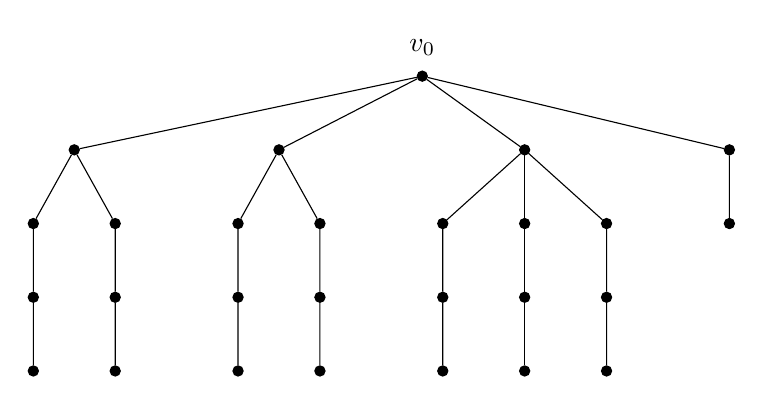
\begin{tikzpicture}[x=0.52cm,y=0.72cm,
  every node/.style={circle,draw,fill=black,inner sep=1.3pt}]
  \node (r) at (10.5,0) {};
  \node (h1) at (2,-1.3) {}; \node (h2) at (7,-1.3) {}; \node (h3) at (13,-1.3) {};
  \node (p1) at (18,-1.3) {}; \node (p2) at (18,-2.6) {};
  \draw (r)--(h1) (r)--(h2) (r)--(h3) (r)--(p1)--(p2);
  \foreach \h/\x in {h1/1,h1/3,h2/6,h2/8,h3/11,h3/13,h3/15}{
    \node (a) at (\x,-2.6) {}; \node (b) at (\x,-3.9) {}; \node (c) at (\x,-5.2) {};
    \draw (\h)--(a)--(b)--(c);
  }
  \node[draw=none,fill=none] at (10.5,0.5) {$v_0$};
\end{tikzpicture}
\caption{The tree $U$ with $27$ vertices.}\label{fig:U}
\end{figure}

\begin{proposition}\label{prop:U}
The tree $U$ satisfies $\gamma(U)=9$ and
\begin{align*}
 D(U,x)={}& 2x^{9}+75x^{10}+2837x^{11}+27278x^{12}+132791x^{13}+403364x^{14}\\
 &+842457x^{15}+1277429x^{16}+1454340x^{17}+1270263x^{18}+862444x^{19}\\
 &+458002x^{20}+190138x^{21}+61213x^{22}+15015x^{23}+2718x^{24}\\
 &+343x^{25}+27x^{26}+x^{27}.
\end{align*}
Since $d_{10}^2=5625<5674=d_{9}d_{11}$, the polynomial $D(U,x)$ is not
log-concave. It is unimodal.
\end{proposition}

\begin{proof}
The polynomial was computed with the recurrence~\eqref{eq:dp} of
Appendix~\ref{app:computation} and confirmed by enumerating all $2^{27}$
subsets of $V(U)$.
\end{proof}

\begin{theorem}\label{thm:unique}
Up to isomorphism, $U$ is the only tree with $27$ vertices whose domination
polynomial is not log-concave.
\end{theorem}

\begin{proof}
This is again the result of the exhaustive computation described in
Appendix~\ref{app:computation}, which covers the $751\,065\,460$ trees with
$27$ vertices.
\end{proof}

\begin{proof}[Proof of Theorem~\ref{thm:smalltrees-intro}]
Part~(i) is Theorem~\ref{thm:small} and Corollary~\ref{cor:smallforest};
part~(ii) is Proposition~\ref{prop:U} and Theorem~\ref{thm:unique}.
\end{proof}

\begin{remark}\label{rem:mechanism}
The failure of log-concavity for $U$ can be traced to the vertex $v_0$. The
dominating sets of $U$ that contain $v_0$ contribute $2$, $75$ and $1141$ to
$d_9$, $d_{10}$ and $d_{11}$, and these three numbers alone satisfy
$75^2\ge2\cdot1141$. A dominating set that avoids $v_0$ has at least two more
vertices than a minimum dominating set; but as soon as it contains a
neighbour $v_i$ of $v_0$, each of the $k_i$ paths attached to $v_i$ can be
dominated by its middle vertex or by its end vertex. There are $1696$
dominating sets of size $11$ that avoid $v_0$, and
$d_{11}=1141+1696=2837$ exceeds $75^2/2$ by less than one per cent. The same
splitting for the tree $T(2,2,3)$, which has $25$ vertices, gives $d_8=1$,
$d_9=37$ and $d_{10}=552+800=1352$, just below $37^2=1369$.
\end{remark}

\begin{remark}\label{rem:family}
Among the trees $T(k_1,\dots,k_r)$ with $r\le5$ and at most $34$ vertices,
exactly six have a non-log-concave domination polynomial: $T(2,3,3)$ of
order $28$; $T(2,3,4)$ and $T(3,3,3)$ of order $31$; and $T(2,3,5)$,
$T(2,4,4)$ and $T(3,3,4)$ of order $34$. For these trees, as for $U$,
log-concavity fails only at the index $\gamma+1$, and the polynomial is
unimodal. In particular the tree $T_3=T(3,3,3)$, which is not covered
by~\cite[Proposition~1]{BS}, is already not log-concave.
\end{remark}


\section{Concluding remarks}\label{sec:remarks}

\subsection*{Gap five}
For $h=5$, Theorem~\ref{thm:criterion-intro} leaves the forests without
isolated vertices that have at most $33$ vertices and satisfy
$n-\gamma\le19$. By Corollary~\ref{cor:smallforest}, a forest of this kind
with a non-unimodal domination polynomial would have a component with at
least $\MinNonLC$ vertices. An exhaustive treatment of the trees with up to
$33$ vertices is out of reach of the programs used here, and
Proposition~\ref{prop:U} shows that log-concavity can no longer be used as
a substitute for unimodality in this range.

\begin{problem}
Prove that the domination polynomial of every forest $F$ with
$\Gamma(F)-\gamma(F)=5$ is unimodal.
\end{problem}

\subsection*{The size of the jumps}
The proof of Theorem~\ref{thm:main} shows that a graph $G$ has a unimodal
domination polynomial as soon as
\begin{equation}\label{eq:jumpquestion}
  c_{j+1}(G)-c_j(G)\le 2\qquad\text{for all } \gamma(G)<j<n ,
\end{equation}
which, by~\eqref{eq:mean}, is the family of inequalities
$(n-j+1)\,d_{j-1}d_{j+1}\le d_jd_{j+1}+(n-j)\,d_j^2$. In the proof of
Lemma~\ref{lem:jump} the variance $v_j$ is bounded by the largest value
compatible with the range of $a(S)$, which could only be attained by a
distribution concentrated on the two extreme values. This crude step is
responsible for the restriction to gaps of order $\sqrt n$.
The inequalities~\eqref{eq:jumpquestion} hold for every tree with at most
$\MaxOrder$ vertices, the largest value of $c_{j+1}-c_j$ over all these trees
being less than $\MaxJumpValue$, and a heuristic search by simulated annealing
among trees with $34$ to $58$ vertices did not produce a value larger than
$1.31$ (supplementary material). Nevertheless they do not hold for all
trees. For $\gamma\le j\le n$ put
\[
  e_j=j-c_j=(n-j+1)\,\frac{d_{j-1}}{d_j},
\]
the average number of non-critical vertices of a dominating set of size $j$;
then $c_{j+1}-c_j=1+e_j-e_{j+1}$ for $\gamma\le j<n$.

\begin{proposition}\label{prop:jumps}
\begin{enumerate}
\item[\textup{(i)}] Let $F$ be a forest of order $n$ and let
$\gamma(F)<j<n$. Then $c_{j+1}-c_j<2\bigl(j-\gamma(F)\bigr)+1$.
\item[\textup{(ii)}] For every integer $t\ge1$ and every $\varepsilon>0$ there
is a tree $T$ such that $c_{j+1}(T)-c_j(T)>2t+1-\varepsilon$ for
$j=\gamma(T)+t$.
\end{enumerate}
In particular, \eqref{eq:jumpquestion} fails for some trees, and the
differences $c_{j+1}-c_j$ are not bounded over all trees.
\end{proposition}

\begin{proof}
(i) By Lemma~\ref{lem:lower}, $j-a(S)\le2(j-\gamma)$ for every
$S\in\Dom_j(F)$, hence $e_j\le2(j-\gamma)$; and $e_{j+1}>0$ because $d_j>0$
and $j<n$.

(ii) Let $r=t+2\ge3$. For integers $k,M\ge1$ let $W$ be the tree obtained from
$T(k,\dots,k)$, with $r$ entries, by attaching to $v_0$ exactly $M$ pendant
paths on two vertices, each joined to $v_0$ by one of its end vertices; it
has $n=1+r+3rk+2M$ vertices. Root $W$ at $v_0$ and
apply~\eqref{eq:dp}. A pendant path on three vertices attached to
$v_i$ has $(A+B+C,\;A+B,\;B)=\bigl(x(x+1)(x+2),\;x(x^2+3x+1),\;x(x+1)\bigr)$
at its end vertex adjacent to $v_i$, and a pendant path on two vertices
attached to $v_0$ has $(A+B+C,\;A+B,\;B)=\bigl(x(x+2),\;x(x+2),\;x\bigr)$.
Writing
\[
  f=x\bigl((x+1)(x+2)\bigr)^k+(x^2+3x+1)^k,\qquad g=f-(x+1)^k,\qquad
  w=(x^2+3x+1)^k-(x+1)^k ,
\]
we obtain $A_{v_i}+B_{v_i}+C_{v_i}=x^kf$, $A_{v_i}+B_{v_i}=x^kg$ and
$B_{v_i}=x^kw$ for $1\le i\le r$, and therefore
\begin{equation}\label{eq:W}
  D(W,x)=x^{rk+M}\Bigl((x+2)^M\bigl(xf^r+g^r\bigr)-w^r\Bigr).
\end{equation}
Here $f(0)=1$, while $g$ and $w$ have zero constant term and linear
coefficients $2^k+2k$ and $2k$. Put $\Phi=(x+2)^Mf^r$ and let $[x^s]\Phi$
denote the coefficient of $x^s$. Since $r\ge3$, \eqref{eq:W} gives
$\gamma(W)=rk+M+1$ and
\begin{equation}\label{eq:Wlow}
  d_{\gamma+s}=[x^s]\Phi\quad(0\le s\le r-2),\qquad
  d_{\gamma+r-1}=[x^{r-1}]\Phi+2^M(2^k+2k)^r-(2k)^r\ \ge\ 2^{M+rk}.
\end{equation}
For $i\ge1$ the coefficient of $x^i$ in $f$ is at most
$2^k\binom{2k}{i-1}+2^i\binom{2k}{i}\le2^k(4k)^i$, because
$(x+1)(x+2)\le2(1+x)^2$ and $x^2+3x+1\le(1+2x)^2$ coefficientwise. Expanding
$f^r$ and noting that at most $\min(i,r)$ factors contribute a positive power
of $x$, we get $[x^i]f^r\le2^{r+i}(4k)^i2^{ki}$ for $1\le i\le r$. From this point assume $M>r-1$, which holds for all sufficiently large $k$
in the choice below. Consequently, for $0\le s\le r-1$,
\[
  [x^s]\Phi=\sum_{i=0}^{s}[x^i]f^r\binom{M}{s-i}2^{M-s+i}
  =\binom Ms2^{M-s}\bigl(1+\theta_s\bigr),\qquad
  0\le\theta_s\le2^r\sum_{i=1}^{s}\Bigl(\frac{16\,k\,s\,2^k}{M-s}\Bigr)^{i},
\]
where we used $\binom{M}{s-i}\big/\binom Ms\le\bigl(s/(M-s)\bigr)^i$. Now let
$k\to\infty$ with $M=2^{k+\lceil k/(2r-2)\rceil}$, so that $k2^k/M\to0$ and
$M^{r-1}/2^{rk}\to0$; then $\theta_s\to0$ for each $s\le r-1$. Let $j=\gamma+t$,
where $t=r-2$, and recall that $n-\gamma=M+2rk+r$. By~\eqref{eq:Wlow},
\[
  e_j=(n-j+1)\frac{d_{\gamma+t-1}}{d_{\gamma+t}}
     =(M+2rk+r-t+1)\,\frac{2t}{M-t+1}\cdot\frac{1+\theta_{t-1}}{1+\theta_t}
     \longrightarrow2t ,
\]
\[
  e_{j+1}=(n-j)\frac{d_{\gamma+t}}{d_{\gamma+t+1}}
     \le(M+2rk+r)\,\frac{M^{t}\,2^{M-t}(1+\theta_t)}{2^{M+rk}}
     \longrightarrow0 .
\]
Hence $c_{j+1}-c_j=1+e_j-e_{j+1}\to2t+1$.
\end{proof}

For $t=1$ the proposition says that $c_{\gamma+2}-c_{\gamma+1}<3$ for every
forest and that the constant $3$ cannot be replaced by a smaller one. The
dominating sets of $W$ of size $\gamma+s$ with $s\le r-2$ are, up to a
negligible proportion, the minimum dominating sets with $s$ further vertices
added on the pendant paths at $v_0$, and each such vertex makes two vertices
non-critical; the far more numerous dominating sets of size $\gamma+r-1$ that
avoid $v_0$ are minimal. Explicitly, the tree obtained from $T(8,8,9)$ by
attaching $3211$ pendant paths on two vertices to $v_0$ has $6501$ vertices
and satisfies $c_{\gamma+2}-c_{\gamma+1}>2$, and for $r=3$, $k=9$ and
$M=7700$ the tree $W$ has $15\,485$ vertices and
$c_{\gamma+2}-c_{\gamma+1}>2.15$. For both trees the complete domination
polynomial was computed from~\eqref{eq:dp}, without the use
of~\eqref{eq:W}; it is unimodal, and \eqref{eq:jumpquestion} fails only for
$j=\gamma+1$ (supplementary material). Trees assembled from the same pieces
are used in~\cite{DHP} for a different purpose: there, a new vertex is joined
to the vertex $v_0$ of each of $m$ copies of $T(k,k,k)$ and to an end vertex
of a path on two vertices, and for large $k$ log-concavity fails at the
indices $\gamma+1,\gamma+3,\dots,\gamma+2m-1$.

The proof of Theorem~\ref{thm:main} uses~\eqref{eq:jumpquestion} only for
indices beyond the increasing segment of Corollary~\ref{cor:segments}(i),
whereas the large jumps of Proposition~\ref{prop:jumps} occur immediately
after $\gamma$. This suggests the following weaker question.

\begin{question}\label{q:jump}
Let $T$ be a tree of order $n$. Does $c_{j+1}(T)-c_j(T)\le2$ hold for every
$j$ with $(n+2\gamma(T)+1)/3<j<n$?
\end{question}

A positive answer would imply the unimodality conjecture for trees, by the
proof of Theorem~\ref{thm:main}. For every tree with at most $26$
vertices, and for the trees $W$ mentioned above, the differences $c_{j+1}-c_j$
in this range are in fact smaller than~$1$ (supplementary material).

At the upper end of this range the answer is positive. Let $T$ be a tree of
order $n\ge5$ with $L$ leaves; then $\gamma(T)\le n/2<n-2$. Clearly
$c_n-c_{n-1}=-c_{n-1}\le0$, and we claim that
\begin{equation}\label{eq:top}
  c_{n-1}-c_{n-2}\le1-\frac2n ,
\end{equation}
with equality if and only if $T$ is a star. A set of vertices is dominating if
and only if its complement contains no closed neighbourhood. The closed
neighbourhoods with two elements are those of the leaves, and they are
pairwise distinct, so $d_{n-2}=\binom n2-L$. Each of them is contained in
$n-2$ sets of three vertices, and a set of three vertices contains at most
two of them, namely when two leaves have the same neighbour. Hence at least
$L(n-2)-\binom L2$ sets of three vertices contain a closed neighbourhood, that
is, $d_{n-3}\le u$ with $u=\binom n3-L(n-2)+\binom L2$. Put $b=d_{n-2}$. Since
$d_{n-1}=n$, \eqref{eq:mean} gives $e_{n-1}=2b/n$ and $e_{n-2}=3d_{n-3}/b$, so
that \eqref{eq:top} is equivalent to $3n\,d_{n-3}\le2b(b-1)$, and
\[
  2b(b-1)-3nu=\tfrac12\,(n-1-L)\bigl(L(3n-4)+n(n-2)\bigr)\ge0 ,
\]
because $L\le n-1$. The right-hand side vanishes only if $L=n-1$, that is,
for the star $K_{1,n-1}$, for which $d_{n-3}=u$.

\subsection*{Beyond forests}
Theorem~\ref{thm:main} applies to every graph satisfying
$(\mathrm{H}_h)$. By Lemma~\ref{lem:upper} and~\eqref{eq:alpha-Gamma}, the upper
bound in~\eqref{eq:H} holds with $h=\Gamma(G)-\gamma(G)$ for every bipartite
graph $G$, so that only the lower bound $a(S)\ge2\gamma(G)-|S|$ is specific to
forests. It fails for $C_4$, but it would be interesting to describe the
bipartite graphs for which it holds.



\subsection*{Supplementary information}
The supplementary material contains the source code of the two programs
described in Appendix~\ref{app:computation} together with their complete
outputs, the auxiliary scripts mentioned in the text, and the Lean~4 sources
described in Appendix~\ref{app:lean}.

\begin{appendices}
%% Appendices (shared).
\section{The computations}\label{app:computation}

This appendix describes the computation behind Theorems~\ref{thm:small}
and~\ref{thm:unique}. All
arithmetic is exact integer arithmetic; no floating-point comparison enters
any of the reported checks.

\subsection*{The recurrence}
Let $T$ be a tree rooted at a vertex $\rho$, and for a vertex $v$ let $T_v$
be the subtree induced by $v$ and its descendants. Consider the subsets $S$
of $V(T_v)$ such that every vertex of $T_v$ other than $v$ is in $S$ or has a
neighbour in $S$. Let $A_v$, $B_v$ and $C_v$ be the generating polynomials, by
cardinality, of those among these sets for which, respectively, $v\in S$;
$v\notin S$ and some child of $v$ is in $S$; $v\notin S$ and no child of $v$
is in $S$. If $v$ is a leaf, then $(A_v,B_v,C_v)=(x,0,1)$, and otherwise,
with $w$ running over the children of $v$,
\begin{equation}\label{eq:dp}
  A_v=x\prod_w(A_w+B_w+C_w),\qquad
  B_v=\prod_w(A_w+B_w)-\prod_w B_w,\qquad
  C_v=\prod_w B_w .
\end{equation}
Indeed, if $v\in S$ the children are unconstrained; if $v\notin S$, every
child must be dominated inside its own subtree, and $C_v$ collects the sets in
which no child is chosen. The root must be dominated, so
$D(T,x)=A_\rho+B_\rho$.

\subsection*{Two programs}
The computation was performed twice, by programs written independently of
each other.

\emph{Program I} generates all rooted trees of order $n$ as level sequences
by the algorithm of Beyer and Hedetniemi~\cite{BH}, and checks that their
number is the number $r_n$ of rooted trees given by the classical recurrence
$(n-1)r_n=\sum_{j=1}^{n-1}\bigl(\sum_{d\mid j}d\,r_d\bigr)r_{n-j}$. It
keeps the rooted trees whose root is a centroid; when the tree has two
centroids, the two rootings are compared through a canonical code and one of
them is kept. Every tree is therefore processed exactly once, and the program
checks that the number of trees processed equals the number
\[
  t_n=r_n-\tfrac12\Bigl(\sum_{k=1}^{n-1}r_kr_{n-k}-[\,n\text{ even}\,]\,r_{n/2}\Bigr)
\]
of trees of order $n$ given by Otter's formula~\cite{Otter}. The domination
polynomial is computed by merging the children of a vertex one at a time,
which is~\eqref{eq:dp} in the equivalent form
$(A,B,C)\mapsto\bigl(A(A_w+B_w+C_w),\,B(A_w+B_w)+CA_w,\,CB_w\bigr)$ starting
from $(x,0,1)$. For every tree of order at most $16$ the program also
enumerates all vertex subsets and compares the resulting numbers of
dominating sets and the values of $\gamma$ and $\Gamma$ with those obtained
from the recurrences (the program computes $\Gamma$ as the independence
number, cf.~\eqref{eq:alpha-Gamma}), and it checks the two
inequalities~\eqref{eq:twosided} for every dominating set; there are $32\,507$ such trees and no
discrepancy.

\emph{Program II} generates the trees of order $n$ directly, by the
algorithm of Wright, Richmond, Odlyzko and McKay~\cite{WROM}, checks their
number against $t_n$, and evaluates~\eqref{eq:dp} as written.

Both programs test $d_j^2\ge d_{j-1}d_{j+1}$ for all $1\le j\le n-1$ with
128-bit integer products; the coefficients themselves are smaller than
$2^{27}$ in the range considered. For each order, both programs also output the
sum, modulo $2^{64}$, of a 64-bit hash of the coefficient vector over all
trees of that order. These sums agree for every order from $2$ to $\MaxOrder$,
which shows, up to hash collisions, that the two programs computed the same
multiset of polynomials although they traverse the trees in different orders
and with different rootings.

\subsection*{Results}
Table~\ref{tab:counts} lists the numbers of trees. Together with the tree on
one vertex, whose domination polynomial is $x$, these are the $\TotalTreesAll$
trees with at most $\MaxOrder$ vertices. Both programs report
that the domination polynomial is log-concave for every tree with at most
$\MaxLC$ vertices, and that exactly one tree with $\MinNonLC$ vertices, the
tree $U$ of Figure~\ref{fig:U}, fails to have this property. Both programs
also report that all these domination polynomials are unimodal.

\begin{table}[ht]
\centering
\caption{Numbers $r_n$ of rooted trees generated by Program~I and numbers
$t_n$ of trees examined by both programs.}\label{tab:counts}
\smallskip
\begin{tabular}{rrr@{\qquad\qquad}rrr}
\hline
$n$ & $r_n$ & $t_n$ & $n$ & $r_n$ & $t_n$\\
\hline
2 & 1 & 1 & 15 & 87\,811 & 7\,741\\
3 & 2 & 1 & 16 & 235\,381 & 19\,320\\
4 & 4 & 2 & 17 & 634\,847 & 48\,629\\
5 & 9 & 3 & 18 & 1\,721\,159 & 123\,867\\
6 & 20 & 6 & 19 & 4\,688\,676 & 317\,955\\
7 & 48 & 11 & 20 & 12\,826\,228 & 823\,065\\
8 & 115 & 23 & 21 & 35\,221\,832 & 2\,144\,505\\
9 & 286 & 47 & 22 & 97\,055\,181 & 5\,623\,756\\
10 & 719 & 106 & 23 & 268\,282\,855 & 14\,828\,074\\
11 & 1\,842 & 235 & 24 & 743\,724\,984 & 39\,299\,897\\
12 & 4\,766 & 551 & 25 & 2\,067\,174\,645 & 104\,636\,890\\
13 & 12\,486 & 1\,301 & 26 & 5\,759\,636\,510 & 279\,793\,450\\
14 & 32\,973 & 3\,159 & 27 & 16\,083\,734\,329 & 751\,065\,460\\
\hline
\end{tabular}

\end{table}

The source code of both programs, their complete outputs, a script that
recomputes the number in Remark~\ref{rem:boundary}, and a program that
enumerates all subsets of a given tree (used for
Proposition~\ref{prop:U}) are contained in the supplementary material.

\section{Formal verification}\label{app:lean}

The following statements have been formalised and checked in
Lean~4 (version 4.27.0) with Mathlib~\cite{Lean,Mathlib}. In the formal
development a graph is a term of Mathlib's type \texttt{SimpleGraph} on a
finite vertex type, a forest is an acyclic graph, and the numbers $\gamma$
and $\Gamma$ are specified by explicit witnesses and bounds rather than by a
defined invariant; for example, $\gamma$ is a natural number such that some
dominating set has at most $\gamma$ elements and every dominating set has at
least $\gamma$ elements.

\begin{itemize}
\item Lemma~\ref{lem:lower}
(\lean{forest_critical_inequality}) and Lemma~\ref{lem:upper}
(\lean{bipartite_critical_le_two_independence}).
\item The core of Theorem~\ref{thm:main}
(\lean{graph_uniform_gap_unimodal}): for an arbitrary relation on a
finite type, natural numbers $h<K$ with $(h+1)^2\le4K$, and an index $A$ with
$\gamma+K\le A+2\le n$ up to which the coefficients are nondecreasing,
condition $(\mathrm{H}_h)$ implies unimodality.
\item Corollary~\ref{cor:gapthree} for forests without isolated vertices and
gap exactly three (\lean{forest_gap_three_unimodal_no_isolates}).
\item Theorem~\ref{thm:criterion-intro}(i) for $h=4$
(\lean{forest_gap_four_large_unimodal}), and the fact that a graph
without isolated vertices that has a minimal dominating set of size
$\gamma+4$ satisfies $n\ge\gamma+14$ or $n\le22$
(\lean{no_isolates_gap_four_large_or_at_most_twenty_two}).
\end{itemize}

All these theorems depend only on the three standard axioms of Lean's
classical logic (\lean{propext}, \texttt{Classical.choice},
\texttt{Quot.sound}). The formalisation does \emph{not} cover the reduction to
forests without isolated vertices (Lemma~\ref{lem:isolates}), the statement
of Theorem~\ref{thm:criterion-intro} for general $h$ in the form given here,
Lemma~\ref{lem:product}, or any part of the computation of
Appendix~\ref{app:computation}. In particular, Theorems~\ref{thm:small} and~\ref{thm:unique}, and
with the former the case of gap four of Theorem~\ref{thm:gapfour-intro}, are
computer-assisted results in the usual sense and not formally verified ones.
The Lean sources are part of the supplementary material.


\end{appendices}

\begin{thebibliography}{99}

\bibitem{AP} Alikhani, S., Peng, Y.-H.: Introduction to domination polynomial of a graph. Ars Combin. \textbf{114}, 257--266 (2014).

\bibitem{BB21} Beaton, I., Brown, J.I.: The average order of dominating sets of a graph. Discrete Math. \textbf{344}(12), 112595 (2021). \url{https://doi.org/10.1016/j.disc.2021.112595}

\bibitem{BB22} Beaton, I., Brown, J.I.: On the unimodality of domination polynomials. Graphs Combin. \textbf{38}(3), 90 (2022). \url{https://doi.org/10.1007/s00373-022-02487-x}

\bibitem{BS} Beaton, I., Schoonhoven, S.: On the unimodality of nearly well-dominated trees. Preprint at \url{https://arxiv.org/abs/2411.02288} (2024)

\bibitem{BH} Beyer, T., Hedetniemi, S.M.: Constant time generation of rooted trees. SIAM J. Comput. \textbf{9}(4), 706--712 (1980). \url{https://doi.org/10.1137/0209055}

\bibitem{BO} Burcroff, A., O'Brien, G.: Unimodality and monotonic portions of certain domination polynomials. Discrete Math. \textbf{346}(9), 113508 (2023). \url{https://doi.org/10.1016/j.disc.2023.113508}

\bibitem{CFPT} Cockayne, E.J., Favaron, O., Payan, C., Thomason, A.G.: Contributions to the theory of domination, independence and irredundance in graphs. Discrete Math. \textbf{33}(3), 249--258 (1981). \url{https://doi.org/10.1016/0012-365X(81)90268-5}

\bibitem{Lean} de Moura, L., Ullrich, S.: The Lean 4 theorem prover and programming language. In: Automated Deduction -- CADE 28, Lecture Notes in Comput. Sci. 12699, Springer, Cham, pp. 625--635 (2021). \url{https://doi.org/10.1007/978-3-030-79876-5_37}

\bibitem{DHP} Du, A., Heilman, S., Panova, G.: Trees and graphs with non log-concave dominating set sequence via AI tools. Preprint at \url{https://arxiv.org/abs/2605.02193} (2026)

\bibitem{GZ} Galvin, D., Zhang, Y.: The domination polynomial of powers of paths and cycles. Preprint at \url{https://arxiv.org/abs/2408.12731} (2024)

\bibitem{KL} Kadrawi, O., Levit, V.E.: The independence polynomial of trees is not always log-concave starting from order 26. Ars Math. Contemp. \textbf{25}(4), \#P4.03 (2025). \url{https://doi.org/10.26493/1855-3974.3207.2ad}

\bibitem{Mathlib} The mathlib Community: The Lean mathematical library. In: Proceedings of the 9th ACM SIGPLAN International Conference on Certified Programs and Proofs (CPP 2020), ACM, New York, pp. 367--381 (2020). \url{https://doi.org/10.1145/3372885.3373824}

\bibitem{Omar} Omar, M.: New perspectives on the unimodality of domination polynomials. Preprint at \url{https://arxiv.org/abs/2601.14494} (2026)

\bibitem{Ore} Ore, O.: Theory of Graphs. Amer. Math. Soc. Colloq. Publ. 38, American Mathematical Society, Providence, RI (1962).

\bibitem{Otter} Otter, R.: The number of trees. Ann. of Math. (2) \textbf{49}(3), 583--599 (1948). \url{https://doi.org/10.2307/1969046}

\bibitem{Stanley} Stanley, R.P.: Log-concave and unimodal sequences in algebra, combinatorics, and geometry. Ann. New York Acad. Sci. \textbf{576}, 500--535 (1989). \url{https://doi.org/10.1111/j.1749-6632.1989.tb16434.x}

\bibitem{WROM} Wright, R.A., Richmond, B., Odlyzko, A., McKay, B.D.: Constant time generation of free trees. SIAM J. Comput. \textbf{15}(2), 540--548 (1986). \url{https://doi.org/10.1137/0215039}

\end{thebibliography}


\section*{Statements and Declarations}
\subsection*{Funding}
No funding was received for conducting this study.

\subsection*{Competing interests}
The author has no relevant financial or non-financial interests to disclose.

\subsection*{Data and code availability}
All data generated during this study, and the code that produced them, are
included in the supplementary material.

\subsection*{Use of AI tools}
Large language model assistants were used in this work to search for
proofs, to write the computer programs and the Lean code, and to draft the
text. The author has checked all arguments and takes full responsibility for
the content.

\end{document}
